% Options for packages loaded elsewhere
\PassOptionsToPackage{unicode}{hyperref}
\PassOptionsToPackage{hyphens}{url}
%
\documentclass[
]{article}
\usepackage{amsmath,amssymb}
\usepackage{iftex}
\ifPDFTeX
  \usepackage[T1]{fontenc}
  \usepackage[utf8]{inputenc}
  \usepackage{textcomp} % provide euro and other symbols
\else % if luatex or xetex
  \usepackage{unicode-math} % this also loads fontspec
  \defaultfontfeatures{Scale=MatchLowercase}
  \defaultfontfeatures[\rmfamily]{Ligatures=TeX,Scale=1}
\fi
\usepackage{lmodern}
\ifPDFTeX\else
  % xetex/luatex font selection
\fi
% Use upquote if available, for straight quotes in verbatim environments
\IfFileExists{upquote.sty}{\usepackage{upquote}}{}
\IfFileExists{microtype.sty}{% use microtype if available
  \usepackage[]{microtype}
  \UseMicrotypeSet[protrusion]{basicmath} % disable protrusion for tt fonts
}{}
\makeatletter
\@ifundefined{KOMAClassName}{% if non-KOMA class
  \IfFileExists{parskip.sty}{%
    \usepackage{parskip}
  }{% else
    \setlength{\parindent}{0pt}
    \setlength{\parskip}{6pt plus 2pt minus 1pt}}
}{% if KOMA class
  \KOMAoptions{parskip=half}}
\makeatother
\usepackage{xcolor}
\usepackage[margin=1in]{geometry}
\usepackage{graphicx}
\makeatletter
\newsavebox\pandoc@box
\newcommand*\pandocbounded[1]{% scales image to fit in text height/width
  \sbox\pandoc@box{#1}%
  \Gscale@div\@tempa{\textheight}{\dimexpr\ht\pandoc@box+\dp\pandoc@box\relax}%
  \Gscale@div\@tempb{\linewidth}{\wd\pandoc@box}%
  \ifdim\@tempb\p@<\@tempa\p@\let\@tempa\@tempb\fi% select the smaller of both
  \ifdim\@tempa\p@<\p@\scalebox{\@tempa}{\usebox\pandoc@box}%
  \else\usebox{\pandoc@box}%
  \fi%
}
% Set default figure placement to htbp
\def\fps@figure{htbp}
\makeatother
\setlength{\emergencystretch}{3em} % prevent overfull lines
\providecommand{\tightlist}{%
  \setlength{\itemsep}{0pt}\setlength{\parskip}{0pt}}
\setcounter{secnumdepth}{-\maxdimen} % remove section numbering
\usepackage{booktabs}
\usepackage{makecell}
\usepackage{float}
\usepackage[section]{placeins}
\usepackage{hyperref}
\hypersetup{colorlinks=true, urlcolor=blue, linkcolor=red}
\usepackage{bookmark}
\IfFileExists{xurl.sty}{\usepackage{xurl}}{} % add URL line breaks if available
\urlstyle{same}
\hypersetup{
  pdftitle={Dimensionality Reduction and Forecast Accuracy: A PCA Approach to Short-Horizon Temperature Prediction},
  hidelinks,
  pdfcreator={LaTeX via pandoc}}

\title{Dimensionality Reduction and Forecast Accuracy: A PCA Approach to
Short-Horizon Temperature Prediction}
\usepackage{etoolbox}
\makeatletter
\providecommand{\subtitle}[1]{% add subtitle to \maketitle
  \apptocmd{\@title}{\par {\large #1 \par}}{}{}
}
\makeatother
\subtitle{FEM11149 - Introduction to Data Science}
\author{Maya Archer 623099 (25\%), Nicolas Gonzalez Gort 780037 (25\%)\\
Rishi Ashok Kumar 560527 (25\%), Saumya Bothra 595402 (25\%)}
\date{}

\begin{document}
\maketitle

\section{Introduction}\label{introduction}

Short horizon temperature forecasts inform planning in energy,
transport, public health, and city services, where load balancing,
maintenance, and emergency response depend on credible next-day
expectations. Utilities, grid operators, and municipalities translate
such forecasts into operational budgets, staffing, and risk management
strategies. Scientifically, multiple drivers shape daily maximum
temperature- surface energy balance (radiative fluxes, cloud cover,
albedo), boundary-layer dynamics (humidity, wind speed, mixing),
seasonal cycles, and urban heat-island effects- the joint behavior of
which exhibits collinearity and regime dependence. Hence, the need to
identify useful predictors for next-day maxima and compress them without
sacrificing accuracy, leading to the central research question of this
study: \emph{To what extent does PCA-based feature extraction improve
next-day maximum-temperature prediction when evaluated out-of-sample and
across different target regimes?} The results of this analysis aim to
clarify which compressed structures carry predictive signal, informs
adoptable model choices for short-horizon operations, and indicates
where forecasts degrade across regimes.

\section{Data}\label{data}

Daily weather observations from the Copernicus Regional Reanalysis for
Europe (CERRA) are used for Rome, yielding 4,020 days (\textasciitilde12
years). The dependent variable is next day daily maximum temperature in
°C. The independent variables include all numeric meteorological
variables observed on day \emph{t}; including the circular angle
\texttt{dominant\_wind\_direction} (0--360°) as is and the same-day
\texttt{max\_temperature\_c} as a lagged regressor for forecasting day
\emph{t+1}. Initial summary statistics show that temperature levels
center around mean 20.90 °C, with average perceived measures averaged at
15.43 °C and average perceived max temperatures at 20.52 °C. Wind
intensity is moderate on average at 15.26 km/h. Average radiative and
evapotranspiration processes show clear seasonality (15.69 MJ/m², 3.03
mm), with photoperiod measures confirming winter--summer contrast- where
the average daylight duration is ≈ 12.21 h. Hydrometeorological activity
averages are low but episodic. Average precipitation lands at 2.44 mm,
where the average rainfall lands at 2.43mm, consistent with many dry
days punctuated by occasional events.

\section{Methodology}\label{methodology}

Some common notation in the following methodolgy are as follows.
\(y_{t}\) denotes the daily maximum temperature (°C) on day \(t\) and
\(X_{t}\in\mathbb{R}^{p}\) is the vector of meteorological predictors
observed on day \(t\). The one day ahead forecasting is done through
supervised regression using aligned pairs
\(\{(X_{t},\,y_{t+1})\}_{t=1}^{T-1}\) in which the response variable is
\(y_{t+1}=\texttt{max\_temperature\_c}\) on the next day, and the
predictors are the full numeric feature set on day \(t\) including the
same-day \texttt{max\_temperature\_c} as a lagged regressor and the
circular angle \texttt{dominant\_wind\_direction} (0--360°) included
untransformed.

The baseline linear model which also serves as the benchmark in this
analysis is an Ordinary Least Squares (OLS) model \[
y_{t+1}=\beta_0+\sum_{j=1}^{p}\beta_j X_{t,j}+\varepsilon_{t+1},
\] While OLS provides interpretable results, it is sensitive to
multi-collinearity among meteorological variables (e.g., temperature
levels and perceived temperatures, radiation and evapotranspiration).
The OLS model is trained on the training set and evaluated on the test
set, the demarcation of which is later specified. \(R^2\) and RMSE is
are used for comparison.

A Principal Component Analysis (PCA) is applied on the training
predictors, after centering means and scaling variances. PCA focuses
primarily on de-correlation and dimensional reduction under strong
multi-collinearity, as mentioned above. While it is not tailored to
extremes, it provides an independent basis for stable regression and
clear diagnostics. With training matrix
\(X_{\text{train}}\in\mathbb{R}^{n\times p}\), PCA computes the
decomposition \(X_{\text{train}}=U D V^{\top}\). Columns of \(V\) are
the loadings and the principal component scores are
\(Z=X_{\text{train}}V\). The variance explained by the \(k\) leading
components is \(\text{VAF}_k=\sum_{j=1}^k d_j^2 / \sum_{j=1}^p d_j^2\).
In this study, the diagnostic checks include the scree plot, a
cumulative Variance Acounted For (VAF) curve, biplots for (PC1, PC2) \&
(PC2, PC3), and loading tables to interpret variable groupings.

In order to choose the number of components, three main methods are
applied on the training set- a cumulative VAF threshold at
\(\ge 85\%\)), The Kaiser's rule where eigenvalues \(>1\), and a
parallel (permutation) analysis comparing real eigenvalues to those from
column wise permuted data. The main model also conducts sensitivity
checks at \(k-1\) and \(k+1\), to assess robustness of predictive
results to the retention level.

Sampling variability in \(\text{VAF}_k\) is quantified by nonparametric
bootstrapping, where rows of \(X_{\text{train}}\) are resampled
\(B=1000\) times. PCA is then recomputed on each bootstrap sample, and
\(\text{VAF}_k\) is aggregated to form a sampling distribution. A 95\%
percentile confidence interval is reported. This procedure is performed
on training data to avoid test leakage.

The principal component analysis regresses the response on the first
\(k\) PC scores: \[
y_{t+1}=\alpha_0+\sum_{j=1}^{k}\gamma_j Z_{t,j}+\eta_{t+1},\qquad Z_{t}=X_{t}V_{(:,1:k)}.
\] The rotation \(V\) and training centering/scaling parameters are
frozen and applied to \(X_{\text{test}}\) to obtain test scores before
prediction.

For this analysis, a contiguous 80/20 split is performed. The first 80\%
of aligned pairs form the training set and the final 20\% form the test
set used only once for final evaluation. All data-dependent
transformations such as scaling and PCA rotations are estimated on the
training set and then applied to the test set.

Prior to modeling, linear associations between each predictor in \(X_t\)
and the target \(y_{t+1}\) are examined using Pearson correlations and
scatter plots with OLS trend lines. These diagnostics motivate the use
of PCA and provide context for interpreting early component loading.

The model's predictive accuracy is assessed on the test set using Root
Mean Squared Error (RMSE) as the primary metric and the \(R^2\) is
provided for context. To examine regime dependence, test observations
are partitioned into deciles of the observed \(y_{t+1}\), and the RMSE
by each decile is reported for the OLS and PCA model specifications,
indicating whether errors concentrate in colder or hotter ranges. Random
seeds are set for reproducibility of re-sampling and permutation steps.

\section{Results}\label{results}

Table 1 (Appendix A) shows that next-day maximum temperature is strongly
correlated to same-day thermal conditions: higher current max/mean/min
(and their perceived counterparts) go hand-in-hand with hotter
tomorrows. Seasonal and surface-energy indicators (sunshine, daylight,
shortwave radiation, and reference evapotranspiration) move in the same
direction, pointing to a ``clear, dry, sunny'' pattern that precedes
warmer days. In contrast, precipitation works in the opposite way,
meaning that more hours or larger sums of rain today are followed by
lower next-day temperatures. Wind variables don't show any strong
effects. The scatterplots in Figure 1 confirm these results showing
positive, near-linear trends for temperature and radiation, and downward
slopes for precipitation.

To avoid look-ahead bias, we estimated Principal Components Analysis
only on the training dataset and froze its rotation and scaling. Figure
X shows a sharp elbow with eigenvalues for PC1-PC4 of 8.82, 3.46, 1.59,
1.00, respectively (Table 2). By the third component we already explain
about 82\% of the variance, with only a small gain if a fourth is added
(up to 88\%), which can be seen in Table 3. The two selection rules
point in slightly different directions: Kaiser would keep 4 components,
while parallel analysis (permutation cut-offs) is more conservative with
k = 3. Balancing parsimony and coverage, we adopt 3 components as the
baseline for prediction and treat the fourth as an optional robustness
check.

Table 5 shows the PCA reduction of weather variables into three
interpretable dimensions. The first component acts like a
``seasonality/heat'' axis: it loads in the same direction on actual and
perceived temperatures, sunshine, shortwave radiation, daylight, and
evapotranspiration, with the opposite sign on precipitation, effectively
contrasting warm, sunny, dry days with cool, wet, overcast ones. The
second component reflects precipitation intensity with gustiness,
distinguishing short, heavy rainfall episodes that coincide with
stronger gusts from longer, lighter precipitation under calmer winds.
The third captures wind strength versus warmth, separating windy--cool
from calm--warm conditions and being driven primarily by wind speed and
gusts with lighter temperature contributions. Communalities indicate
that the best-represented variables in the k = 3 subspace are actual and
perceived temperatures (max\_temperature\_c, mean\_temperature\_c,
perceived\_max\_temperature\_c, perceived\_mean\_temperature\_c),
together with radiative and photoperiod indicators
(shortwave\_radiation\_sum\_mj\_m2, daylight\_duration\_s,
sunshine\_duration\_s) and reference\_evapotranspiration\_mm. Snowfall,
precipitation hours, and dominant\_wind\_direction are least
represented. We retain three components because the scree flattens after
the third, the parallel-analysis cutoff aligns with a conservative
choice of three, and cross-validated PCR error improves up to k = 3 with
small gains after. In addition, the first three components together
account for about 82\% of the variance (bootstrap 95\% CI =
81.1--82.1\%), so the dimensionality reduction is reliable and not
driven by a particular sample split.

Table 6 presents the results of our Principal Component Regression (PCR)
on the training set. Cross-validated RMSEP drops from 2.31 to 2.24, and
finally to 2.06 when moving from 1 to 3 components, and changes only
marginally at 4 components (2.05), indicating diminishing returns beyond
k = 3. As a benchmark, we fit a standard multiple linear regression
(OLS) to the original predictors. On the held-out test data, OLS
achieves a lower RMSE (1.80) than PCR with k = 3 (2.16). PCR's \(R^2\)
value is high on both train and test datasets, but the absolute error is
slightly larger than OLS in this split. This suggests that, for this
horizon and feature set, compressing predictors with unsupervised PCA
does not by itself improve point prediction accuracy over a
well-specified linear model. This is consistent with expectations given
(1) the near-linear relations between thermal and radiative predictors
and next-day maxima and (2) inclusion of same-day max\_temperature\_c as
a strong lagged signal that supervised OLS can exploit directly, whereas
unsupervised PCA is not optimized for the target.

Because PCA optimizes total variance, not tail loss, it can under-weight
rare extremes even if those are operationally important. That limitation
motivates our final check: grouping test observations into deciles by
realized next-day heat and plotting RMSE by method. The resulting curves
are broadly similar across deciles (error does not spike dramatically in
specific bins for this split), with OLS generally at or below PCR. Error
profiles are not strongly dependent on the heat level in this split; if
tail fidelity becomes a priority, one could consider quantile or
weighted regression, EVT-informed losses, or nonlinear terms (e.g.,
splines for radiation or seasonality).

\section{Conclusion and Discussion}\label{conclusion-and-discussion}

PCA successfully compressed the weather feature space into three
interpretable dimensions that together explain \textasciitilde82\% of
training variance. The retained components capture a warm--sunny--dry vs
cool--overcast--wet gradient (PC1), a precipitation--gustiness axis
(PC2), and wind strength vs warmth (PC3). However, when evaluated
out-of-sample on a contiguous 20\% test set, the OLS model outperforms
the PCA, with an RSME (≈1.80) lower than PCR (≈2.16). Sensitivity checks
showed diminishing returns beyond 3 principal components, aligning with
the scree/parallel-analysis decision rule. Answering the central
research question, the study finds that PCA-based feature extraction
does not improve next day maximum temperature prediction over a
well-specified linear regression, for this specific horizon, city
(Rome), and split. However, PCA remains valuable for diagnostics,
de-correlation, and compact reporting, but not as a stand-alone route to
lower point-forecast error here.

Two design choices likely shaped this outcome and point to refinements.
First, PCA is unsupervised and it maximizes total variance rather than
temperature predictive variance. Supervised alternatives like OLS may
better exploit signal under collinearity. Under collinearity,
ridge/elastic-net would also be expected to match or exceed PCR by
targeting predictive variance directly while keeping all (ridge) or
grouped (elastic-net) signals. Second, two features merit targeted
treatment: the inclusion of same-day \texttt{max\_temperature\_c} as a
lagged regressor- useful but potentially dominating simpler components-
and circular wind direction, which was included untransformed. Encoding
direction via \(\sin/\cos\) terms can make wind-related structure
legible to linear methods. For robustness, future work should use
rolling-origin evaluation (rather than a single 80/20 split), probe
nonlinearities/interactions (e.g., splines for radiation/seasonality),
and re-test decile performance with an emphasis on extremes.

\subsection{Appendix A}\label{appendix-a}

\begin{table}[H]\centering
\caption{Correlations with Next-day Maximum Temperature}
\label{tab:A1}
\begin{tabular}{lc}
\toprule
Variable & Pearson $r$ \\
\midrule
max\_temperature\_c & 0.969 \\
perceived\_max\_temperature\_c & 0.963 \\
mean\_temperature\_c & 0.956 \\
perceived\_mean\_temperature\_c & 0.950 \\
perceived\_min\_temperature\_c & 0.906 \\
min\_temperature\_c & 0.903 \\
reference\_evapotranspiration\_mm & 0.870 \\
daylight\_duration\_s & 0.779 \\
shortwave\_radiation\_sum\_mj\_m2 & 0.769 \\
sunshine\_duration\_s & 0.649 \\
dominant\_wind\_direction & 0.434 \\
max\_wind\_gusts\_km\_h & 0.120 \\
max\_wind\_speed\_km\_h & 0.005 \\
snowfall\_sum\_mm & $-0.086$ \\
rain\_sum\_mm & $-0.190$ \\
precipitation\_sum\_mm & $-0.195$ \\
precipitation\_hours\_h & $-0.300$ \\
\bottomrule
\end{tabular}
\end{table}

\begin{table}[!htbp]\centering
\caption{PCA Eigenvalues (Training Set)}
\label{tab:A2}
\begin{tabular}{lc}
\toprule
PC & Eigenvalue \\
\midrule
PC1 & 8.825 \\
PC2 & 3.464 \\
PC3 & 1.585 \\
PC4 & 1.004 \\
PC5 & 0.890 \\
PC6 & 0.828 \\
PC7 & 0.547 \\
PC8 & 0.387 \\
PC9--PC17 & $<0.31$ \\
\bottomrule
\end{tabular}
\end{table}

\begin{table}[!htbp]\centering
\caption{Variance Explained by Principal Components (Training Set)}
\label{tab:A3}
\begin{tabular}{lcc}
\toprule
PC & Proportion of Variance & Cumulative Variance \\
\midrule
PC1 & 0.519 & 0.519 \\
PC2 & 0.203 & 0.723 \\
PC3 & 0.093 & 0.816 \\
PC4 & 0.059 & 0.875 \\
PC5 & 0.046 & 0.922 \\
PC6 & 0.040 & 0.962 \\
PC7 & 0.018 & 0.980 \\
PC8 & 0.008 & 0.988 \\
PC9--PC17 & $\approx$ 0.012 (total) & 1.000 \\
\bottomrule
\end{tabular}
\end{table}

\begin{table}[!htbp]\centering
\caption{Parallel Analysis (Training): Real Eigenvalues vs.\ 95\% Cutoffs}
\label{tab:A4}
\begin{tabular}{lccc}
\toprule
PC & Real Eigenvalue & 95\% Cutoff & Keep \\
\midrule
PC1 & 8.825 & $\approx$1.1 & Yes \\
PC2 & 3.464 & $\approx$1.1 & Yes \\
PC3 & 1.585 & $\approx$1.1 & Yes \\
PC4 & 1.004 & $\approx$1.1 &  \\
PC5+ & $<1$ & $\approx$1.1 &  \\
\bottomrule
\end{tabular}
\end{table}

\begin{table}[!htbp]\centering
\caption{PCA Loadings (PC1--PC3, Training Set)}
\label{tab:A5}
\begin{tabular}{lccc}
\toprule
Variable & PC1 & PC2 & PC3 \\
\midrule
mean\_temperature\_c & $-0.32$ & $-0.10$ & 0.13 \\
max\_temperature\_c & $-0.33$ & $-0.04$ & 0.10 \\
min\_temperature\_c & $-0.30$ & $-0.16$ & 0.17 \\
perceived\_mean\_temperature\_c & $-0.32$ & $-0.09$ & 0.19 \\
perceived\_max\_temperature\_c & $-0.32$ & $-0.04$ & 0.16 \\
perceived\_min\_temperature\_c & $-0.30$ & $-0.14$ & 0.21 \\
max\_wind\_speed\_km\_h & 0.01 & $-0.35$ & $-0.56$ \\
max\_wind\_gusts\_km\_h & $-0.03$ & $-0.38$ & $-0.52$ \\
shortwave\_radiation\_sum\_mj\_m2 & $-0.30$ & 0.09 & $-0.20$ \\
dominant\_wind\_direction & $-0.17$ & $-0.10$ & $-0.13$ \\
reference\_evapotranspiration\_mm & $-0.32$ & 0.02 & $-0.18$ \\
daylight\_duration\_s & $-0.29$ & $-0.06$ & $-0.13$ \\
sunshine\_duration\_s & $-0.26$ & 0.20 & $-0.21$ \\
precipitation\_sum\_mm & 0.09 & $-0.46$ & 0.20 \\
snowfall\_sum\_mm & 0.03 & $-0.03$ & $-0.08$ \\
precipitation\_hours\_h & 0.12 & $-0.43$ & 0.16 \\
rain\_sum\_mm & 0.09 & $-0.46$ & 0.21 \\
\bottomrule
\end{tabular}
\end{table}

\begin{table}[!htbp]\centering
\caption{PCR Cross-Validated RMSEP by Number of Components (Training)}
\label{tab:A6}
\begin{tabular}{lc}
\toprule
$k$ & RMSEP (CV) \\
\midrule
1 & 2.305 \\
2 & 2.244 \\
3 & 2.055 \\
4 & 2.052 \\
\bottomrule
\end{tabular}
\end{table}

\begin{table}[!htbp]\centering
\caption{Test Performance: OLS vs.\ PCR ($k=3$)}
\label{tab:A7}
\begin{tabular}{lccc}
\toprule
Model & RMSE (Test) & $R^{2}$ (Train) & $R^{2}$ (Test) \\
\midrule
OLS (All Variables) & 1.800 & --- & --- \\
PCR ($k=3$) & 2.156 & 0.920 & 0.925 \\
\bottomrule
\end{tabular}
\end{table}

\begin{table}[!htbp]\centering
\caption{RMSE by Observed Max-Temperature Decile (Test Set)}
\label{tab:A8}
\begin{tabular}{lcc}
\toprule
Decile Group & RMSE: OLS & RMSE: PCR ($k=3$) \\
\midrule
G1 (coolest) &  &  \\
G2 &  &  \\
G3 &  &  \\
G4 &  &  \\
G5 &  &  \\
G6 &  &  \\
G7 &  &  \\
G8 &  &  \\
G9 &  &  \\
G10 (hottest) &  &  \\
\bottomrule
\end{tabular}
\end{table}

\subsection{Appendix B}\label{appendix-b}

\begin{figure}[H]

{\centering 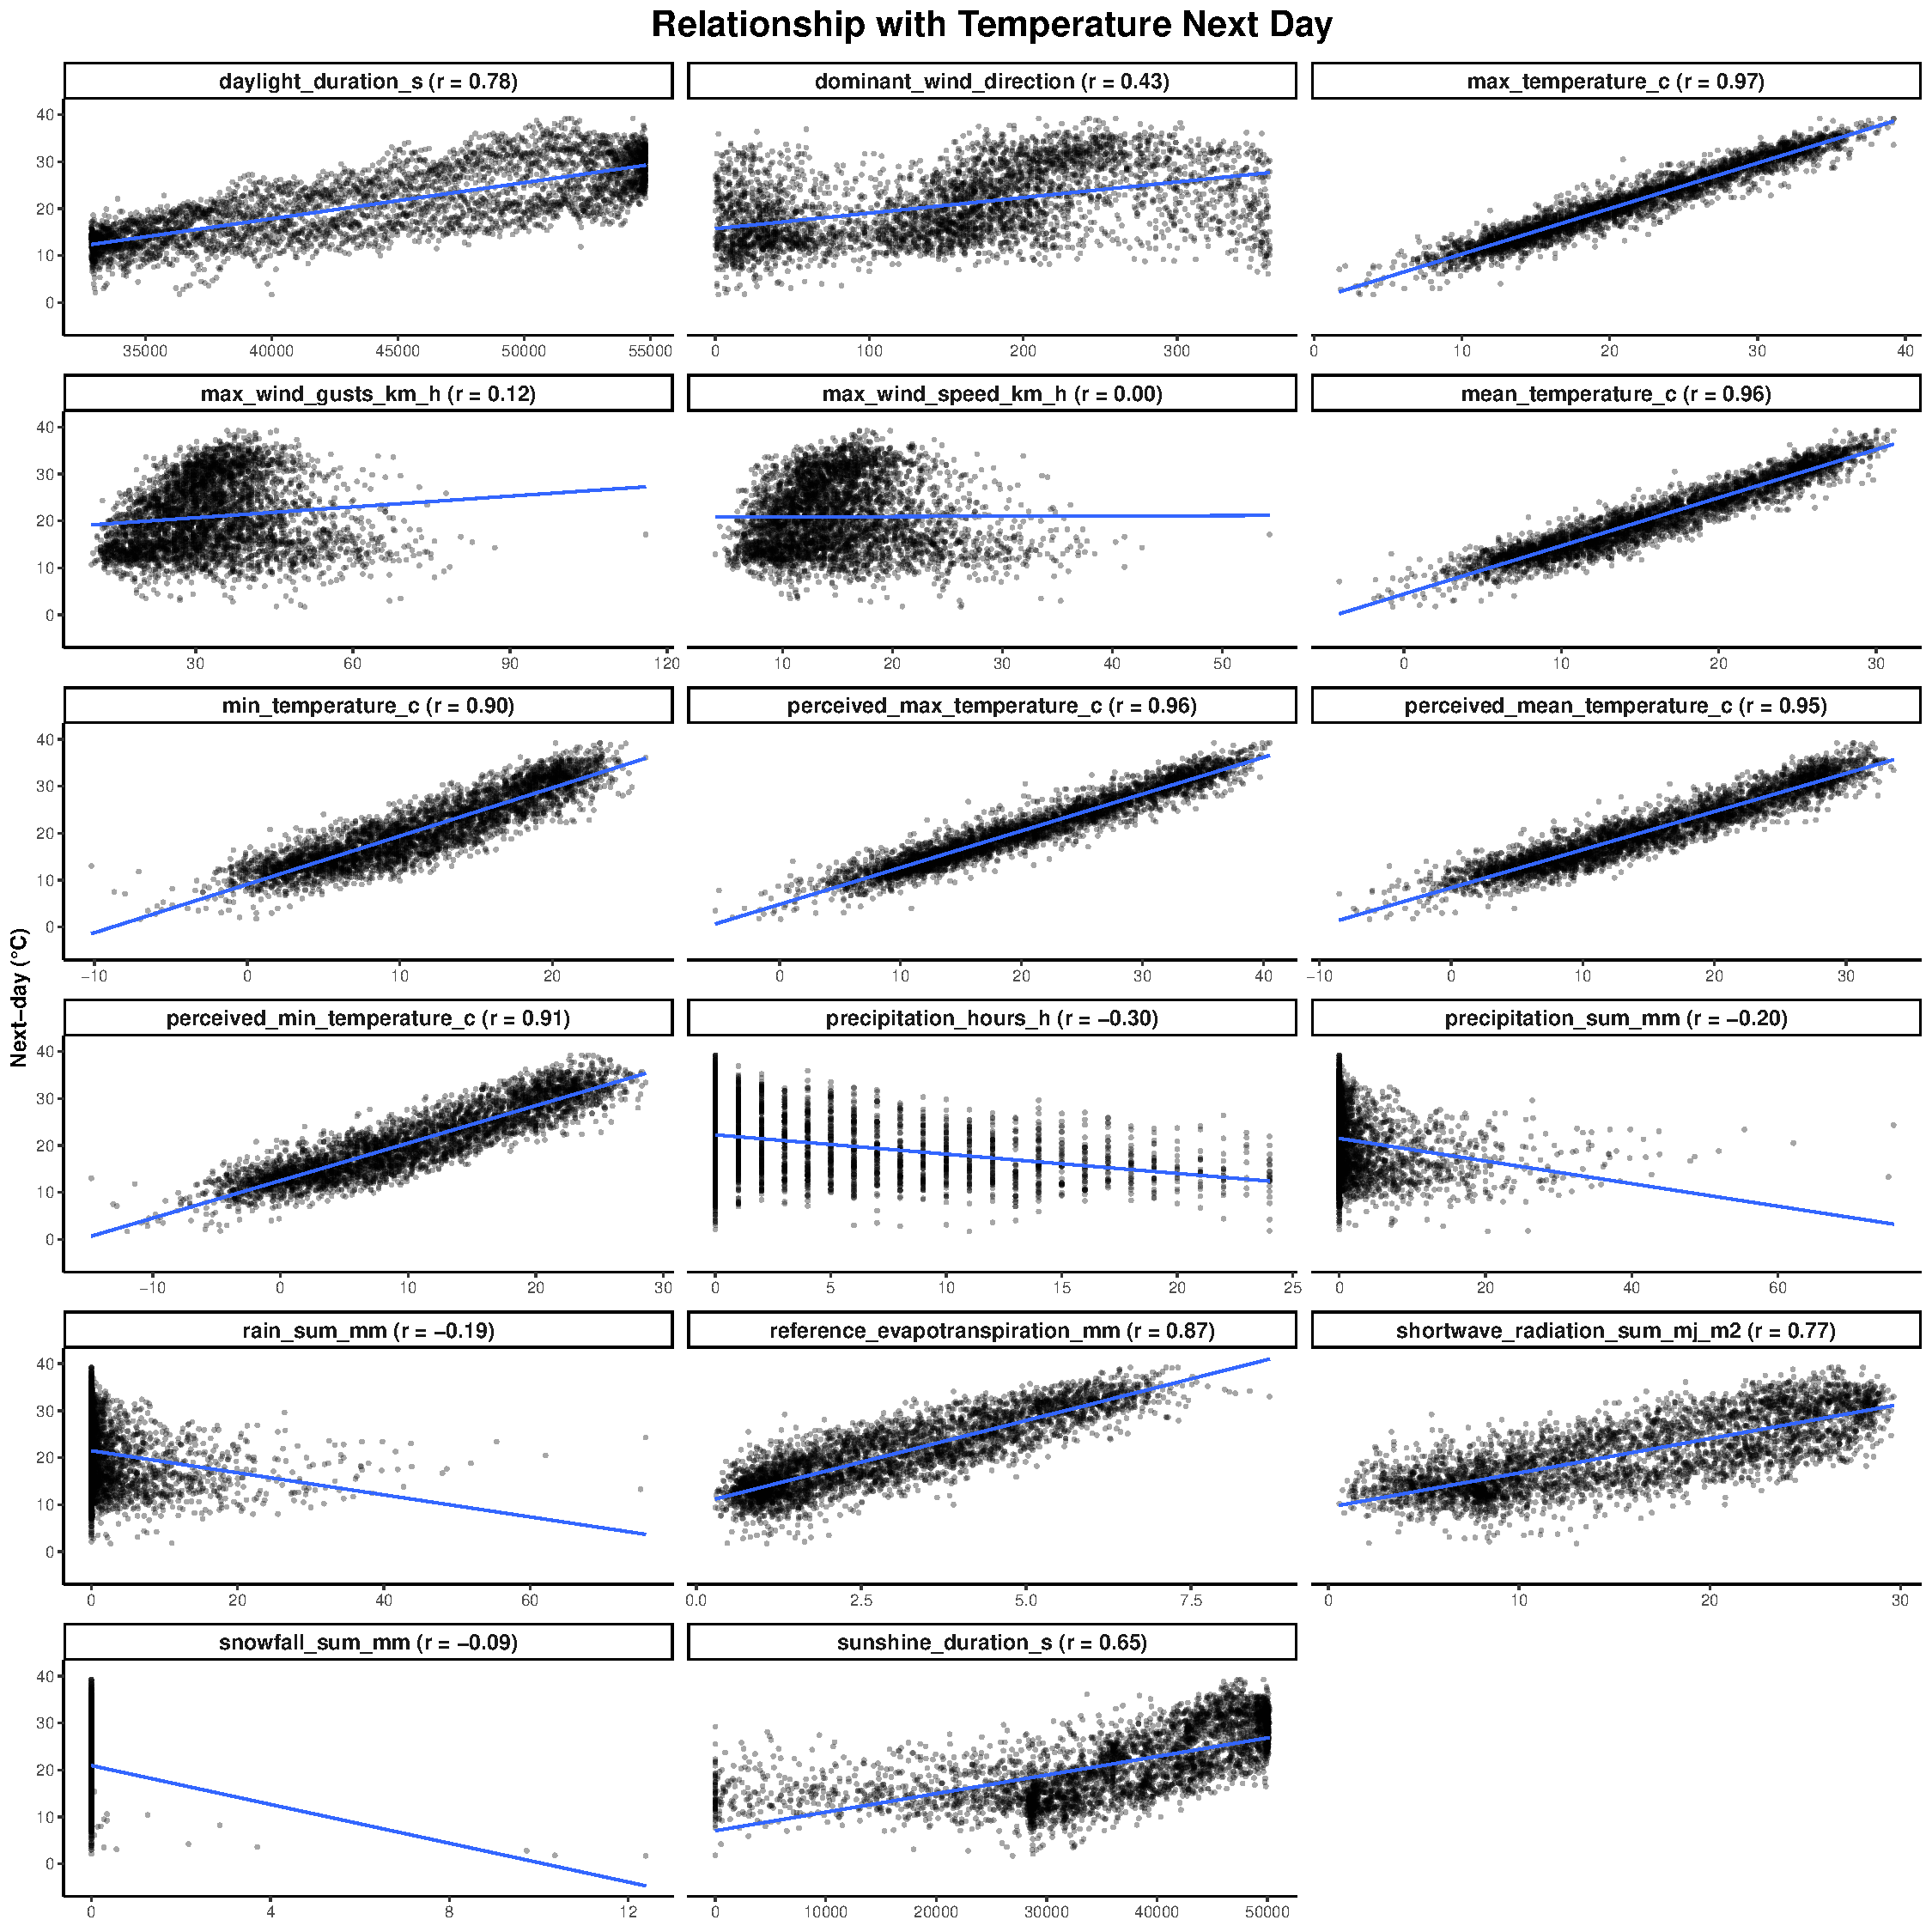
\includegraphics[width=0.8\linewidth]{Assignment2_Group9_files/figure-latex/unnamed-chunk-1-1} 

}

\caption{Scatter Correlations}\label{fig:unnamed-chunk-1}
\end{figure}

\begin{figure}[H]

{\centering 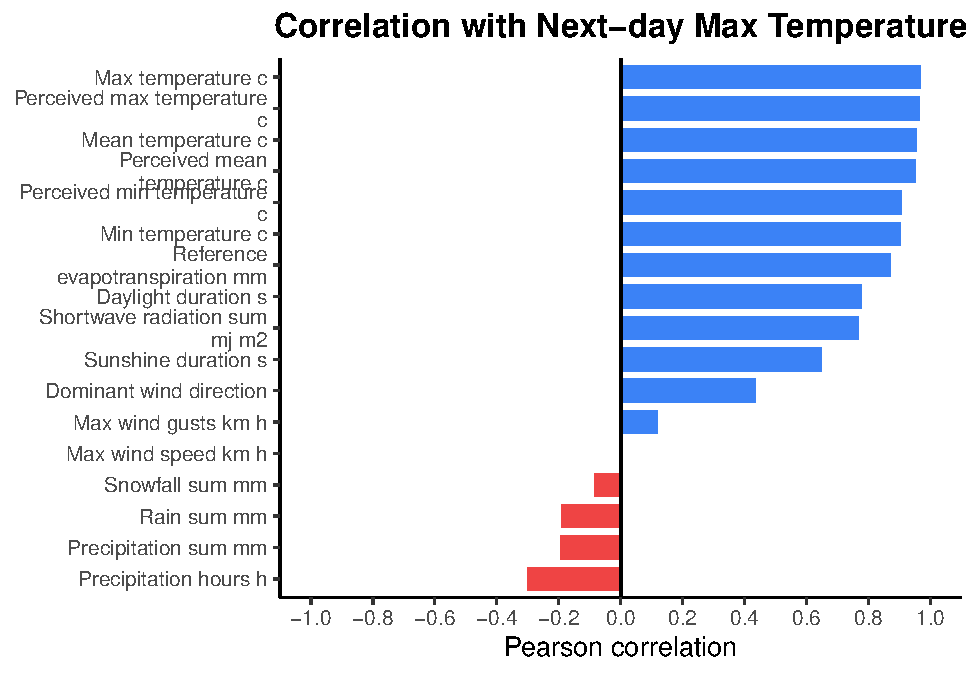
\includegraphics[width=0.8\linewidth]{Assignment2_Group9_files/figure-latex/unnamed-chunk-2-1} 

}

\caption{Pearson Correlation}\label{fig:unnamed-chunk-2}
\end{figure}
\begin{figure}[H]

{\centering 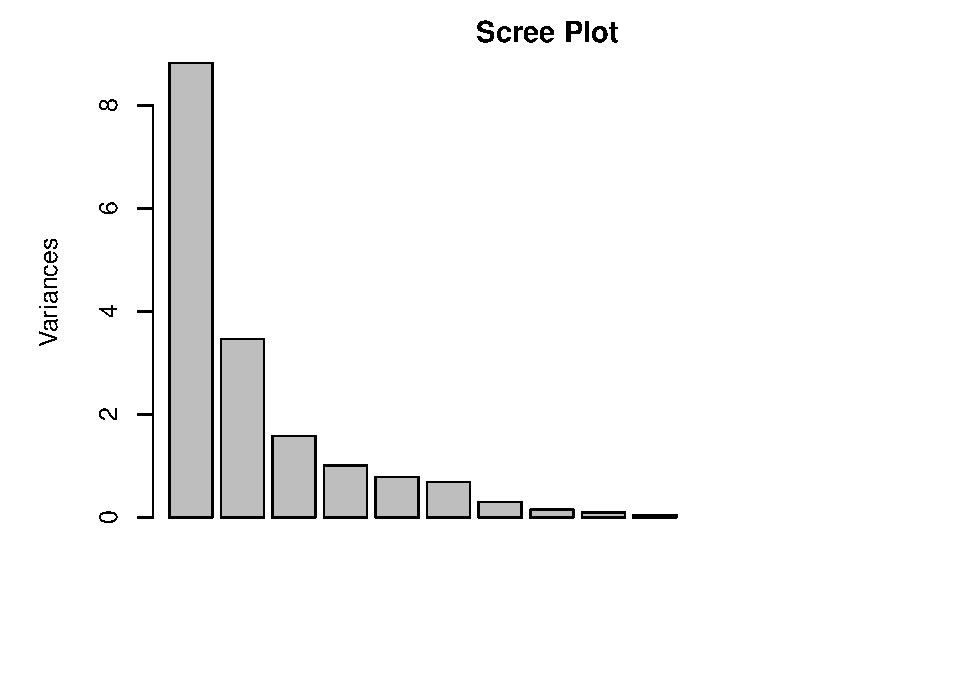
\includegraphics[width=0.8\linewidth]{Assignment2_Group9_files/figure-latex/unnamed-chunk-3-1} 

}

\caption{Scree Plot}\label{fig:unnamed-chunk-3}
\end{figure}
\begin{figure}[H]

{\centering 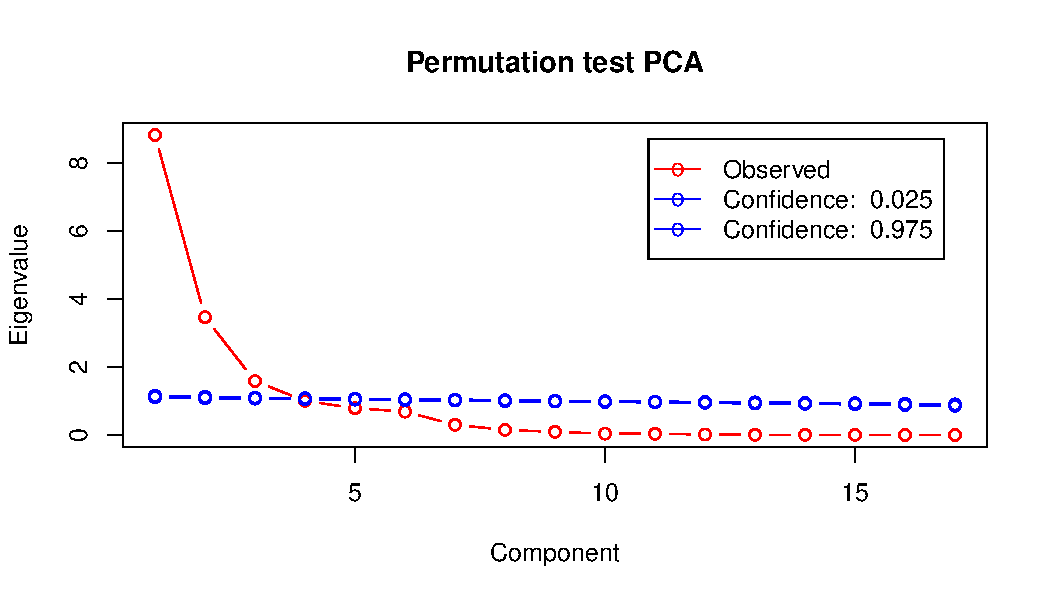
\includegraphics[width=0.8\linewidth]{Assignment2_Group9_files/figure-latex/unnamed-chunk-4-1} 

}

\caption{Permutation Test}\label{fig:unnamed-chunk-4}
\end{figure}

\begin{figure}[H]

{\centering 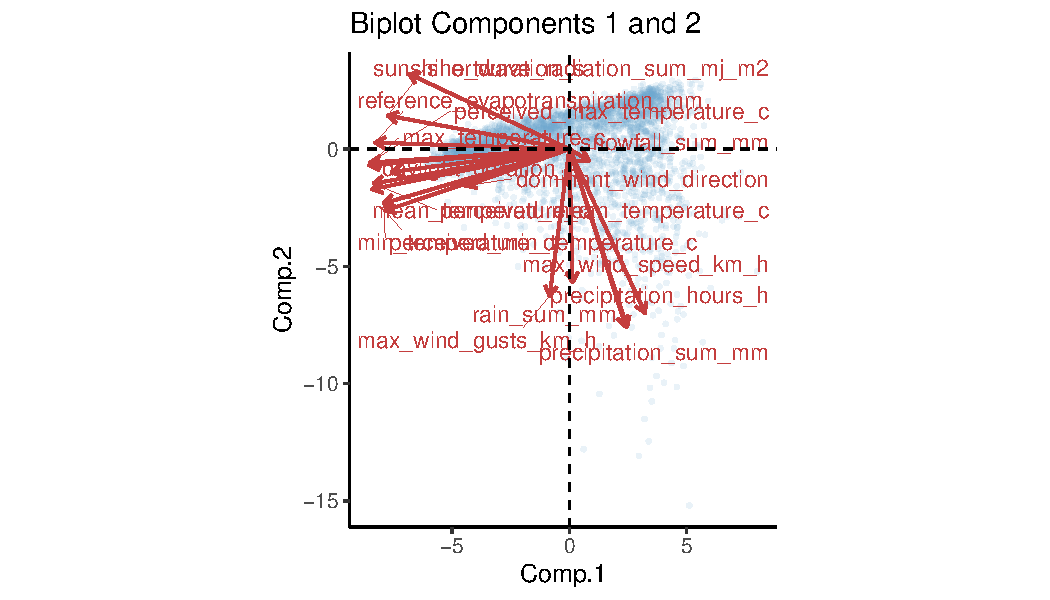
\includegraphics[width=0.8\linewidth]{Assignment2_Group9_files/figure-latex/unnamed-chunk-5-1} 

}

\caption{ Biplot Components 1-2}\label{fig:unnamed-chunk-5}
\end{figure}

\begin{figure}[H]

{\centering 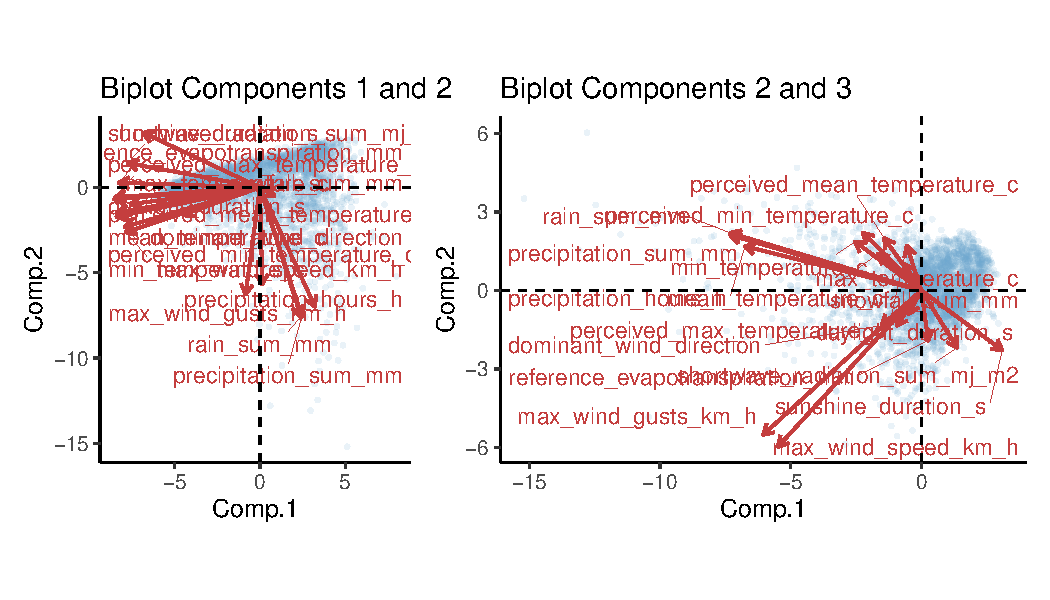
\includegraphics[width=0.8\linewidth]{Assignment2_Group9_files/figure-latex/unnamed-chunk-6-1} 

}

\caption{Biplot all Components}\label{fig:unnamed-chunk-6}
\end{figure}

\begin{figure}[H]

{\centering 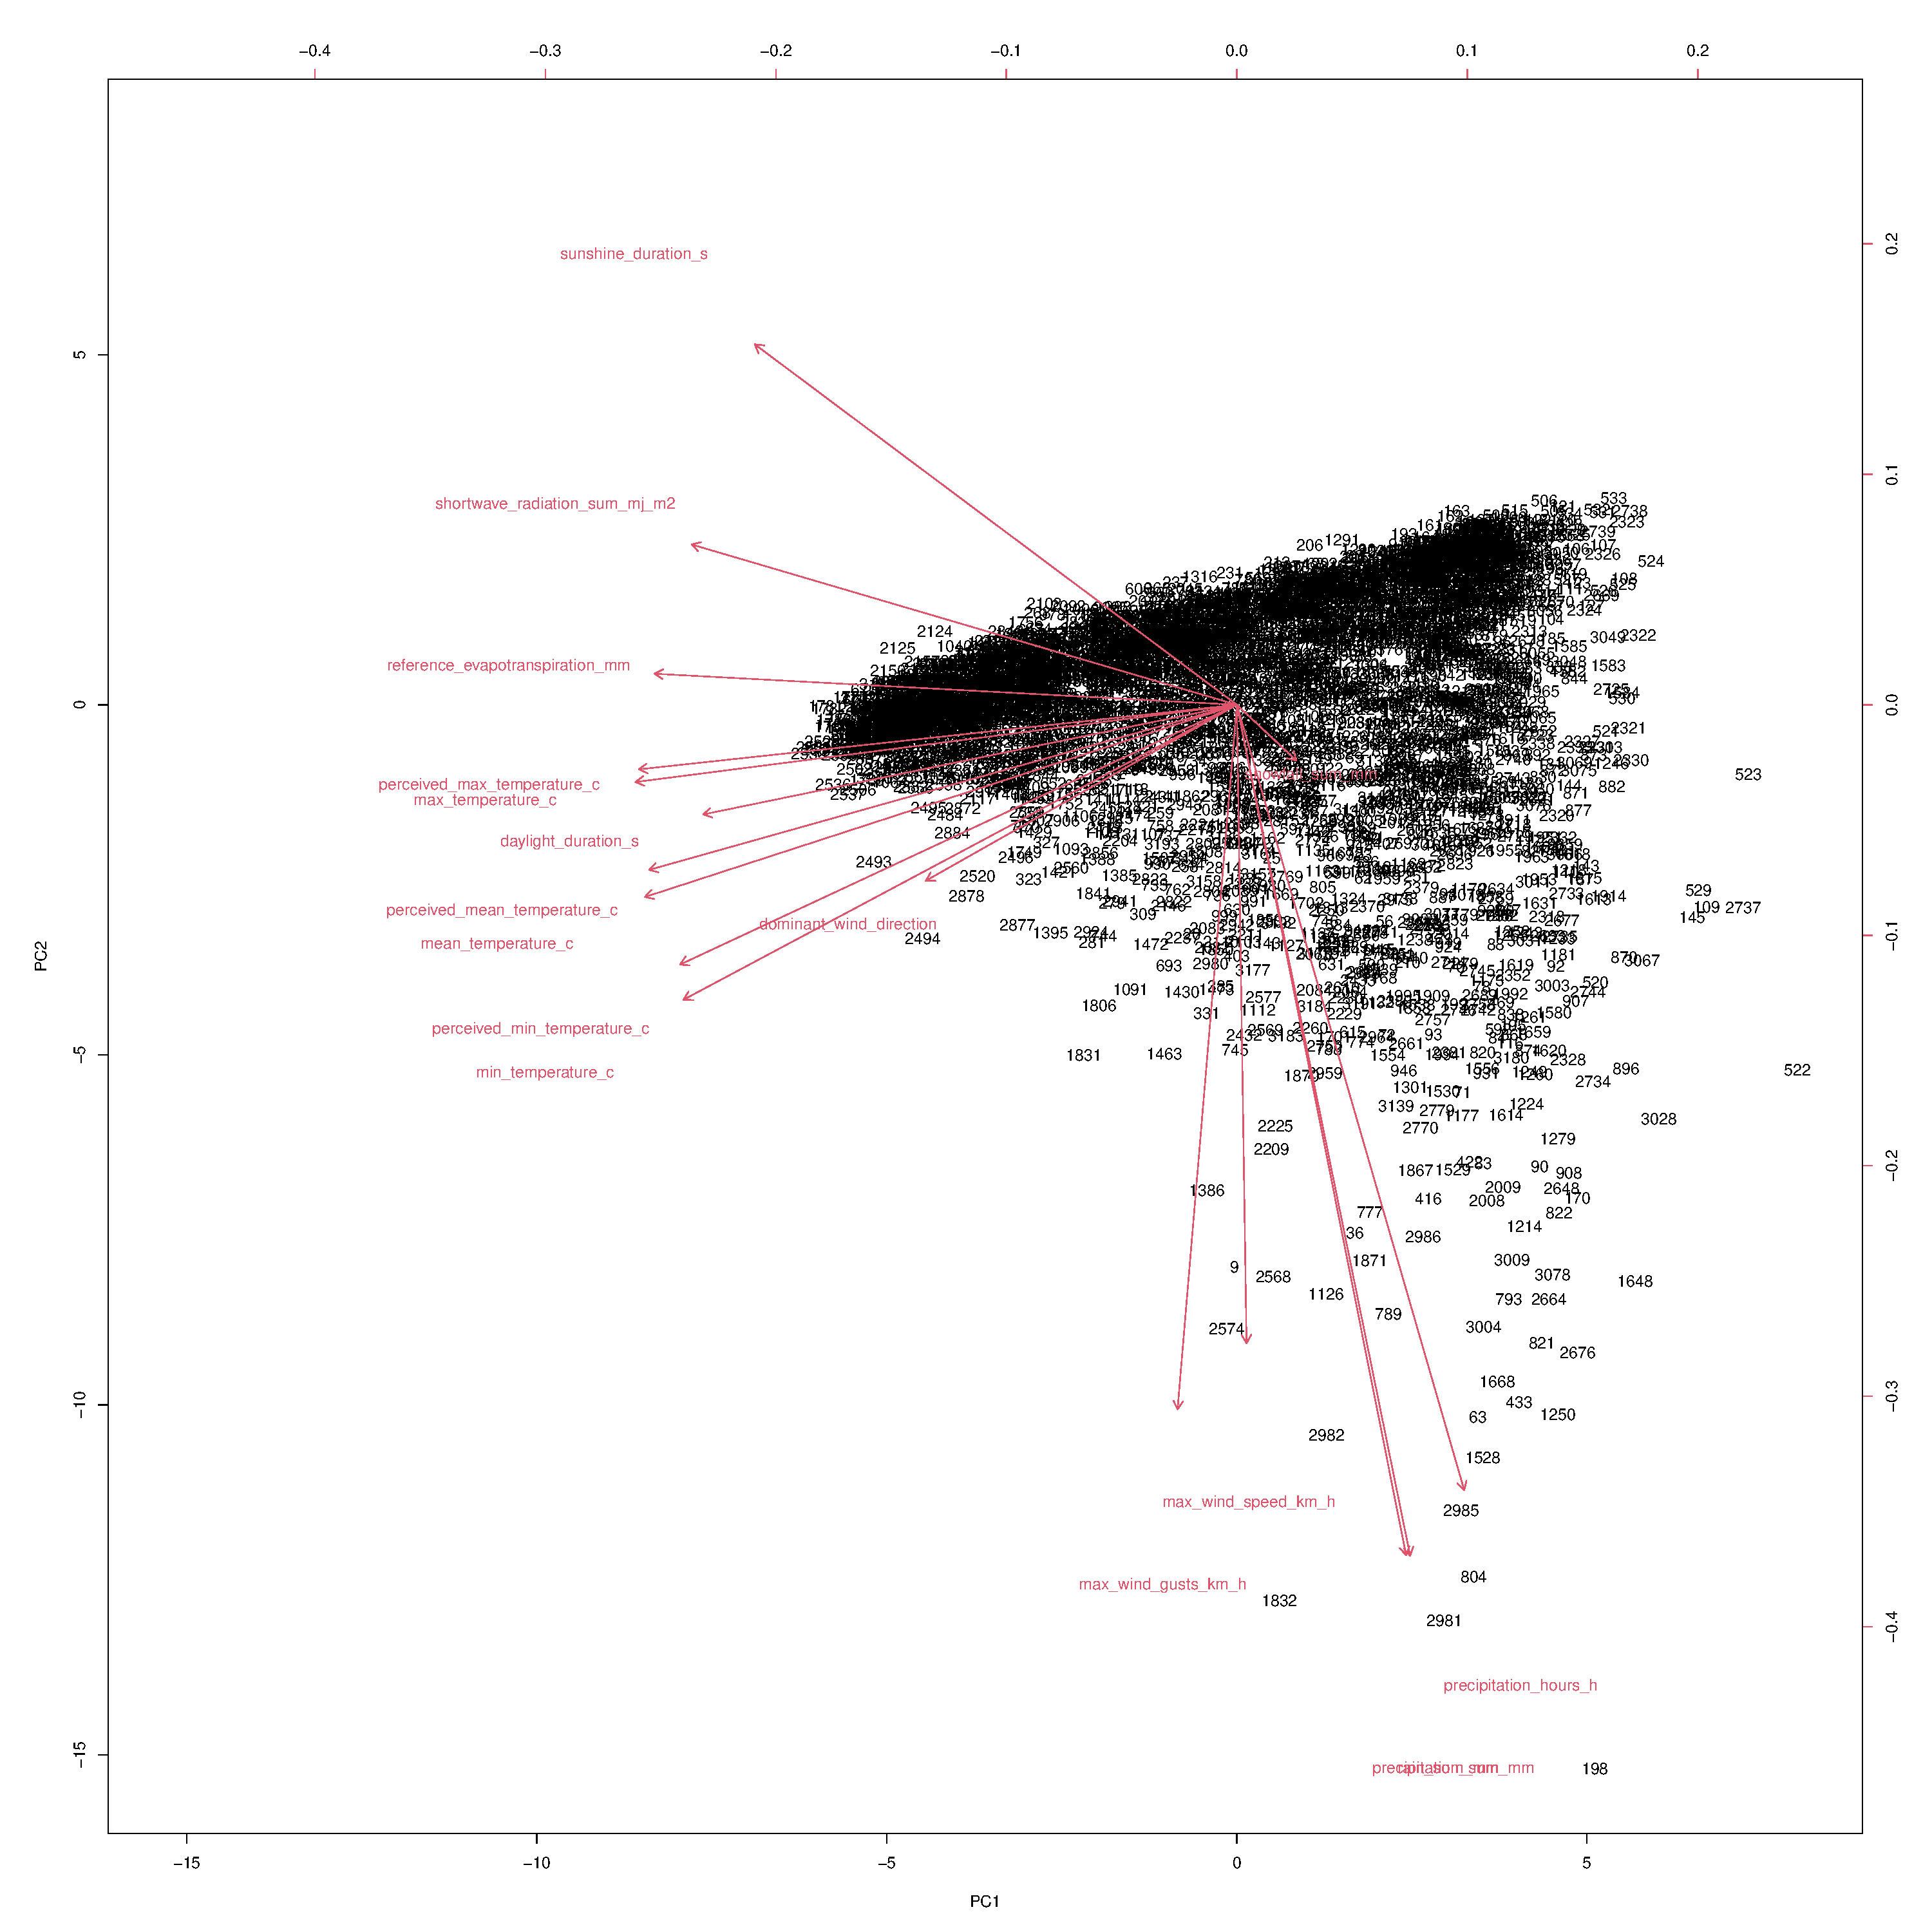
\includegraphics[width=0.8\linewidth]{Assignment2_Group9_files/figure-latex/unnamed-chunk-7-1} 

}

\caption{Biplot of the first two components}\label{fig:unnamed-chunk-7}
\end{figure}
\begin{figure}[H]

{\centering 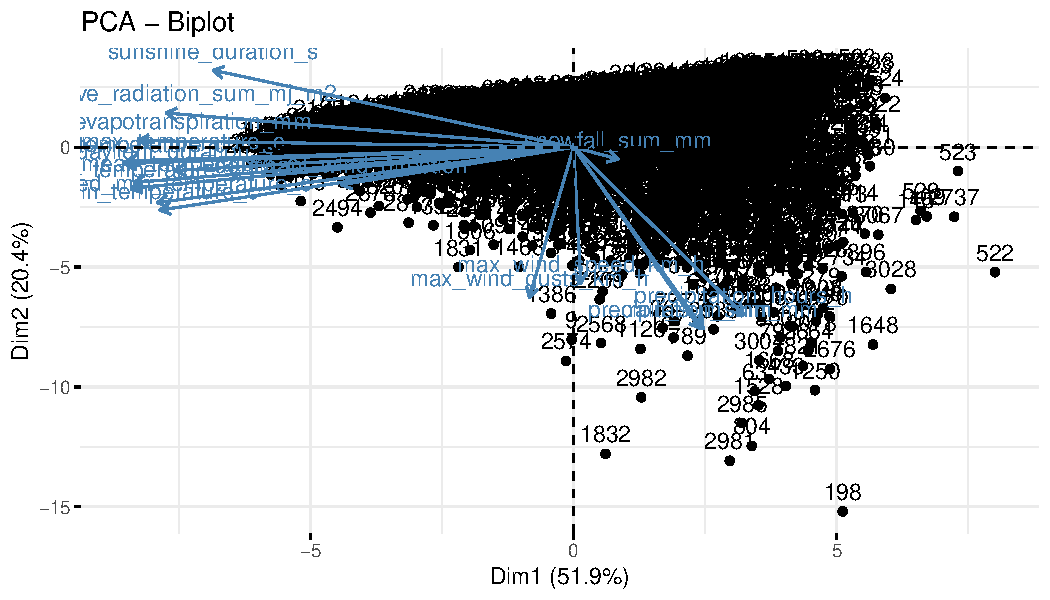
\includegraphics[width=0.8\linewidth]{Assignment2_Group9_files/figure-latex/unnamed-chunk-8-1} 

}

\caption{Optimal Visualization}\label{fig:unnamed-chunk-8}
\end{figure}

\begin{figure}[H]

{\centering 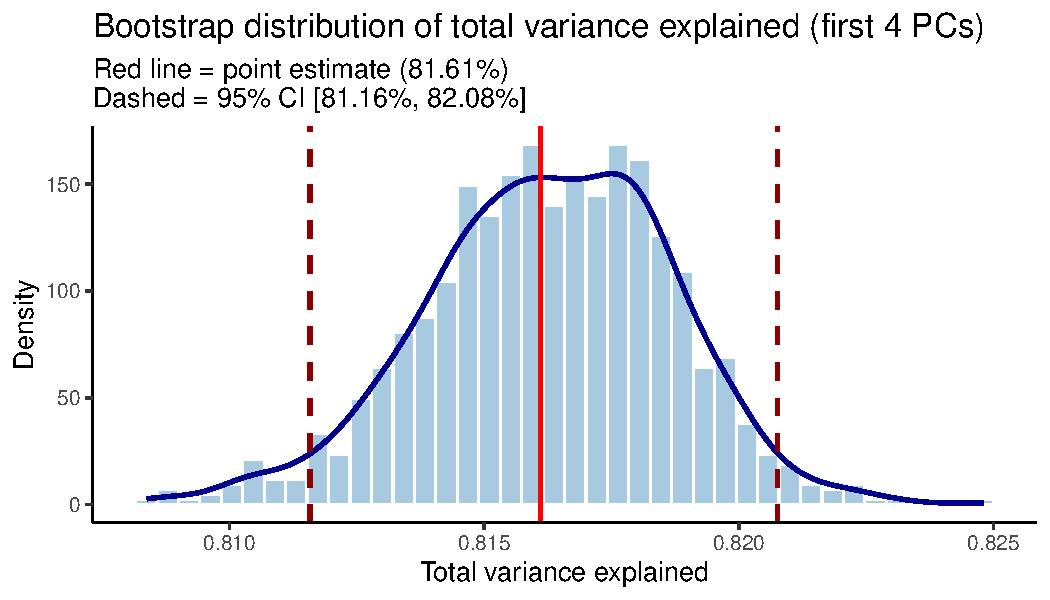
\includegraphics[width=0.8\linewidth]{Assignment2_Group9_files/figure-latex/unnamed-chunk-9-1} 

}

\caption{Plot density + CI + point estimate}\label{fig:unnamed-chunk-9}
\end{figure}

\begin{figure}[H]

{\centering 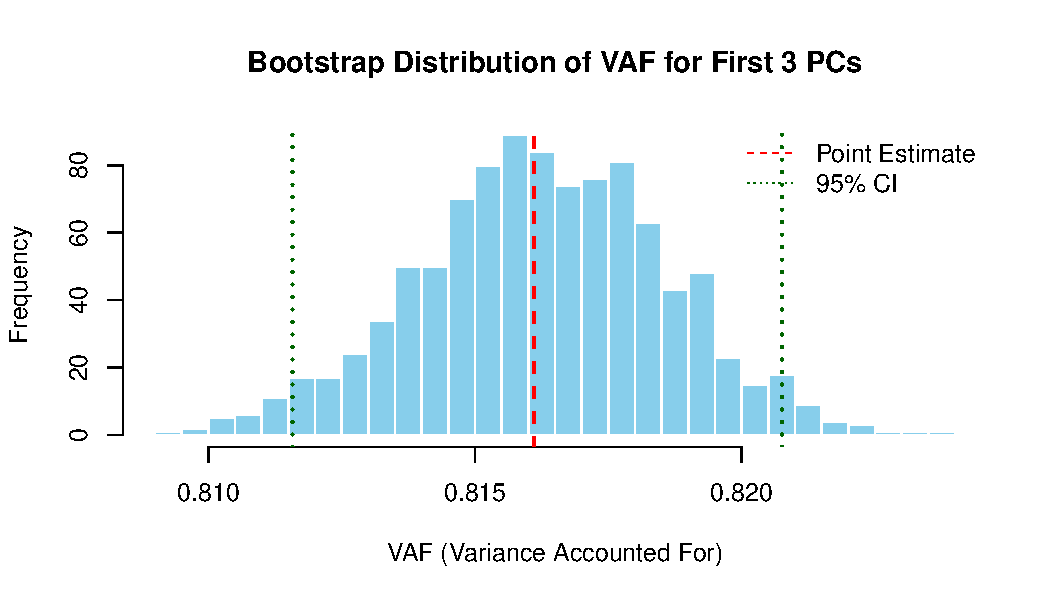
\includegraphics[width=0.8\linewidth]{Assignment2_Group9_files/figure-latex/unnamed-chunk-10-1} 

}

\caption{Boostrap Distribution}\label{fig:unnamed-chunk-10}
\end{figure}

\begin{figure}[H]

{\centering 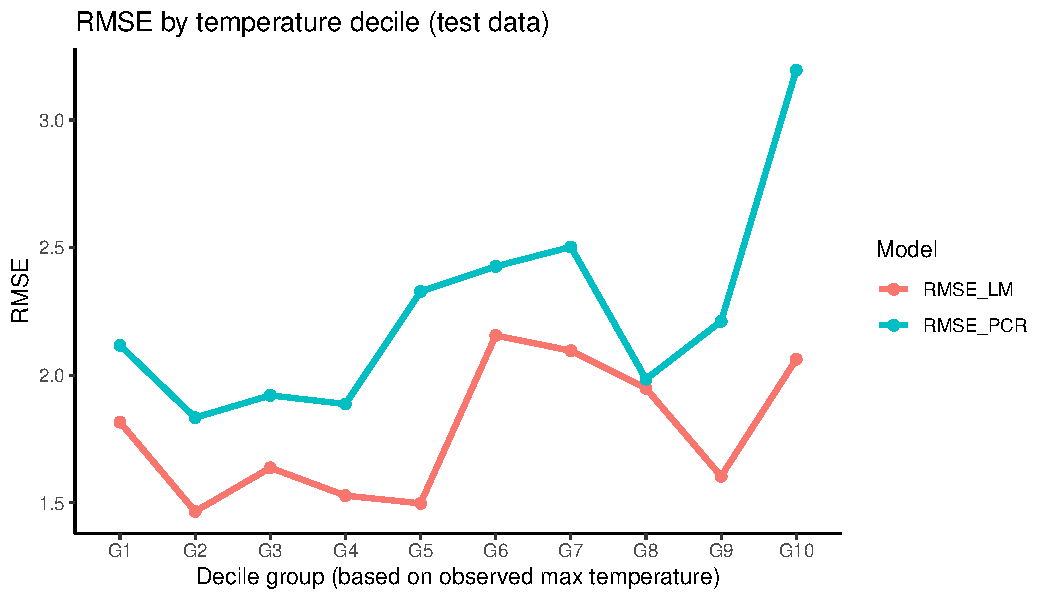
\includegraphics[width=0.8\linewidth]{Assignment2_Group9_files/figure-latex/unnamed-chunk-11-1} 

}

\caption{RMSE by temperature decile}\label{fig:unnamed-chunk-11}
\end{figure}

\subsection{Appendix C}\label{appendix-c}

\begin{verbatim}
## # Appendix C. Full code
\end{verbatim}

\begin{verbatim}
## ```r
\end{verbatim}

\begin{verbatim}
##  knitr::opts_chunk$set(echo=FALSE, message=FALSE, warning=FALSE)
## library(readr)
## library(tidyverse)
## library(janitor)
## library(ggplot2)
## library(dplyr)
## library(stringr)
## rm(list = ls())
## knitr::opts_chunk$set(
##   fig.align = "center",
##   fig.pos = "H",
##   out.width = "80%",
##   fig.width = 7,
##   fig.height = 4,
##   dpi = 300)
## 
## # Directory setup
## #path = dirname(rstudioapi::getSourceEditorContext()$path) # Path is directory of this file
## #setwd(path) 
## # no scientific notations
## options(scipen = 999)
## data <- read.csv("a2_data_group_9.csv")
## names(data)
## 
## # Preprocessing
## data <- janitor::clean_names(data) # cleans all the cols names automatically 
## names(data)
## 
## data <- data %>%
##   select(-location_id)
## # --- 1. Create X and y ---
## 
## # Build the X matrix: all variables, except the last row
## X <- as.matrix(data[-nrow(data), ]) # this includes the date col
## 
## # Build the y vector: the max temperature column, except its first observation
## y <- data$max_temperature_c[-1]
## 
## # Check alignment and dimensions
## dim(X)  # should be (n-1) x p
## length(y)  # should be (n-1)
## # --- 2. Compute correlations ---
## 
## # 0) Ensure all-numeric predictors and aligned X/y
## df_corr <- data %>% dplyr::select(where(is.numeric))
## 
## X_corr <- df_corr[-nrow(df_corr), ]            # data.frame (predictors at time t)
## y_corr <- df_corr$max_temperature_c[-1]        # vector (target at time t+1)
## 
## # 1) Correlations
## correlations <- sapply(X_corr, function(x) cor(x, y_corr, use = "complete.obs"))
## correlations <- sort(correlations, decreasing = TRUE)
## print(correlations)
## 
## # 2) Plot ALL variables
## num_vars <- ncol(X_corr)
## # par(mfrow = c(4, 5))   # 4 rows × 5 columns grid (enough for 17 plots)
## # 
## # for (col in names(correlations)) {
## #   x <- X_corr[[col]]
## #   plot(x, y_corr,
## #        main = paste("M vs", col),
## #        xlab = col,
## #        ylab = "Next-day (°C)",
## #        pch = 19, col = "darkblue")
## #   abline(lm(y_corr ~ x), col = "red", lwd = 2)
## # }
## # 
## # par(mfrow = c(1, 1))  # reset plotting layout
## 
## # 2) Data para facetas (larga)
## vars_ordered <- names(correlations)
## 
## plot_df <- X_corr %>%
##   dplyr::select(all_of(vars_ordered)) %>%
##   mutate(`Next-day (°C)` = y_corr) %>%
##   pivot_longer(cols = all_of(vars_ordered),
##                names_to = "variable",
##                values_to = "x")
## 
## # 3) Etiquetas con r para cada panel
## lab_map <- setNames(
##   paste0(vars_ordered, " (r = ", sprintf("%.2f", correlations), ")"),
##   vars_ordered
## )
## 
## # 4) Gráfico facetado
## p <- ggplot(plot_df, aes(x = x, y = `Next-day (°C)`)) +
##   geom_point(alpha = 0.35, size = 0.6) +
##   geom_smooth(method = "lm", se = FALSE, linewidth = 0.7) +
##   facet_wrap(~ variable,
##              labeller = as_labeller(lab_map),
##              scales = "free_x",
##              nrow = 6) +              
##   labs(
##     title = "Relationship with Temperature Next Day",
##     x = NULL,
##     y = "Next-day (°C)"
##   ) +
##   theme_classic(base_size = 12) +
##   theme(
##     plot.title = element_text(hjust = 0.5, size = 20, face = "bold", margin = margin(b = 10)),
##     strip.text = element_text(size = 12, face = "bold"),
##     axis.text  = element_text(size = 9),
##     axis.title.y = element_text(size = 12, face = "bold"),
##     panel.spacing = unit(8, "pt")
##   )
## 
## 
## # 3) Correlation summary bar chart for the report
## 
## # correlations should already be a named numeric vector
## corr_df <- tibble(
##   variable = names(correlations),
##   corr = as.numeric(correlations)
## ) %>%
##   arrange(desc(corr)) %>%  # positives first, then negatives
##   mutate(
##     label = str_replace_all(variable, "_", " "),
##     label = str_to_sentence(label),
##     label = str_wrap(label, width = 25),
##     label = factor(label, levels = rev(label))  # keep sorted order
##   )
## 
## # # Plot
## # ggplot(corr_df, aes(x = label, y = corr, fill = corr > 0)) +
## #   geom_col(width = 0.75) +
## #   geom_hline(yintercept = 0, color = "black", linewidth = 0.7) +
## #   coord_flip() +
## #   labs(
## #     title = "Correlation with Next-day Max Temperature",
## #     x = NULL,
## #     y = "Pearson correlation"
## #   ) +
## #   scale_fill_manual(values = c("TRUE" = "#3B82F6", "FALSE" = "#EF4444")) +
## #   scale_y_continuous(
## #     limits = c(-1, 1),
## #     breaks = seq(-1, 1, 0.2)
## #   ) +
## #   theme_minimal(base_size = 13) +
## #   theme(
## #     legend.position = "none",      # remove legend
## #     panel.grid.major.y = element_blank(),
## #     panel.grid.minor = element_blank(),
## #     plot.title = element_text(face = "bold", hjust = 0.5),
## #     axis.text.y = element_text(size = 10)
## #   )
## # --- 3. Train Test Split (Time Series) ---
## 
## # 0) Ensure time order
## data <- data %>% arrange(date)
## 
## # 1) Keep only numeric predictors (this automatically drops Date)
## X_df <- data %>% select(where(is.numeric))  # includes max_temperature_c
## 
## # 2) Build aligned X (t) and y (t+1)
## X <- as.matrix(X_df[-nrow(X_df), , drop = FALSE])
## y <- data$max_temperature_c[-1]
## 
## # 3) Time indices (keep separately; do NOT include in X)
## time_X <- data$date[-nrow(data)]
## time_y <- data$date[-1]
## 
## # --- train/test split by proportion, no leakage ---
## n <- nrow(X); k <- floor(0.8 * n)
## X_train <- X[1:k, , drop = FALSE]; y_train <- y[1:k]
## X_test  <- X[(k+1):n, , drop = FALSE]; y_test <- y[(k+1):n]
## # --- 4. Generate PC on X_train ---
## 
## # 1. Perform PCA *only* on training data
## pca_model <- prcomp(X_train, center = TRUE, scale. = TRUE)
## 
## # 2. Check how much variance each component explains
## summary(pca_model)
## 
## # 3. Look at the contribution of each variable to each PC
## round(pca_model$rotation,2)  
## # 2. Eigenvalues (variances of PCs) and explained variance
## eig  <- pca_model$sdev^2
## 
## # Show only eigenvalues > 1 (Kaiser's rule)
## data.frame(
##   PC = paste0("PC", seq_along(eig)),
##   Eigenvalue = eig
## ) %>% 
##   dplyr::filter(Eigenvalue > 1)
## 
## # 3. Using Cumulative VAF
## prop_var <- eig / sum(eig)
## cum_var  <- cumsum(prop_var)
## tau   <- 0.85
## k_vaf <- which(cum_var >= tau)[1]
## k_vaf
## 
## cum_var
## # 4
## source("permtestPCA.R")          # Load the permtestPCA() function
## perm_range <- permtestPCA(X_train)
## 
## dev.new(width = 8, height = 5)
## 
## # --- Permutation (Parallel Analysis) for choosing number of PCs ---
## 
## # X_train: numeric matrix/data.frame (observations x variables)
## # B: number of permutations (e.g., 1000)
## # alpha: significance level for the cutoff (0.05 uses 95th percentile of permuted eigs)
## # Returns a list with suggested k and helpful objects, and draws a scree-style plot.
## perm_parallel_pca <- function(X_train, B = 1000, alpha = 0.05, seed = 42,
##                               center = TRUE, scale. = TRUE, make_plot = TRUE) {
##   stopifnot(is.data.frame(X_train) || is.matrix(X_train))
##   if (!is.null(seed)) set.seed(seed)
##   
##   X <- as.matrix(X_train)
##   n <- nrow(X)
##   p <- ncol(X)
##   
##   # 1) PCA on the real data
##   pca_real <- prcomp(X, center = center, scale. = scale.)
##   eig_real <- pca_real$sdev^2  # length p
##   
##   # 2) Permutation: shuffle rows within each column to break correlation, keep marginals
##   perm_eigs <- replicate(B, {
##     Xb <- apply(X, 2, function(col) sample(col, size = n, replace = FALSE))
##     # PCA on permuted data
##     pb <- prcomp(Xb, center = center, scale. = scale.)
##     pb$sdev^2
##   })
##   
##   perm_eigs <- t(perm_eigs)  # B x p (rows=replicates)
##   
##   # 3) For each component j, get the (1-alpha) quantile across permutations
##   q_perm <- apply(perm_eigs, 2, quantile, probs = 1 - alpha, names = FALSE)
##   
##   # 4) Suggested k: how many components have real eigenvalue > permutation cutoff
##   keep_vec <- eig_real > q_perm
##   k_suggested <- if (any(keep_vec)) max(which(keep_vec)) else 0
##   
##   # 5) Helpful summaries
##   vaf_real <- eig_real / sum(eig_real)
##   cum_vaf_real <- cumsum(vaf_real)
##   vaf_q_perm <- q_perm / sum(eig_real)        # put cutoffs on same scale for plotting
##   cum_vaf_q_perm <- cumsum(vaf_q_perm)
##   
##   # 6) Plot
##   if (make_plot) {
##     op <- par(no.readonly = TRUE); on.exit(par(op), add = TRUE)
##     
##     # Scree with cutoff
##     plot(1:p, eig_real, type = "b", pch = 16,
##          xlab = "Principal component", ylab = "Eigenvalue",
##          main = sprintf("Parallel Analysis (Permutation): suggested k = %d", k_suggested))
##     lines(1:p, q_perm, type = "b", pch = 1)
##     abline(v = k_suggested + 0.5, lty = 3)  # visual separator after chosen k
##     legend("topright",
##            legend = c("Real data eigenvalues", sprintf("Permutation cutoff (%.0f%%)", (1 - alpha) * 100)),
##            pch = c(16, 1), lty = 1, bty = "n")
##   }
##   
##   list(
##     k_suggested = k_suggested,
##     eigen_real = eig_real,
##     eigen_perm = perm_eigs,   # B x p matrix
##     cutoff_quantile = q_perm, # length p (eigenvalue thresholds)
##     keep = keep_vec,          # logical vector of length p
##     vaf_real = vaf_real,
##     cum_vaf_real = cum_vaf_real
##   )
## }
## 
## perm_range <- perm_parallel_pca(X_train)
## 
## # Biplot of first 2 PCs
## # biplot(pca_model, scale = 0)
## 
## library(factoextra)
## library(ggplot2)
## library(patchwork)
## 
## # --- If your dataset is huge, optionally downsample *for plotting only* ---
## set.seed(1)
## plot_idx <- seq_len(min(4000, nrow(X_train)))  # or sample.int(nrow(X_train), 4000)
## pca_plot <- prcomp(X_train[plot_idx, , drop = FALSE], center = TRUE, scale. = TRUE)
## 
## # A. PC1 vs PC2
## p12 <- fviz_pca_biplot(
##   pca_plot,
##   axes = c(1, 2),
##   label = "var",           # only label variables
##   repel = TRUE,             # avoid overlap
##   col.var = "#C43E3E",     # red loadings
##   arrowsize = 0.7,
##   col.ind = "skyblue3",    # points
##   alpha.ind = 0.15,         # transparency
##   pointsize = 0.6
## ) +
##   coord_fixed() +
##   theme_classic(base_size = 12) +
##   theme(
##     panel.grid.minor = element_blank(),
##     legend.position = "none"
##   ) +
##   labs(title = "Biplot Components 1 and 2", x = "Comp.1", y = "Comp.2")
## # p12
## 
## # B. PC2 vs PC3
## p23 <- fviz_pca_biplot(
##   pca_plot,
##   axes = c(2, 3),
##   label = "var",
##   repel = TRUE,
##   col.var = "#C43E3E",
##   arrowsize = 0.7,
##   col.ind = "skyblue3",
##   alpha.ind = 0.15,
##   pointsize = 0.6
## ) +
##   coord_fixed() +
##   theme_classic(base_size = 12) +
##   theme(
##     panel.grid.minor = element_blank(),
##     legend.position = "none"
##   ) +
##   labs(title = "Biplot Components 2 and 3", x = "Comp.1", y = "Comp.2")
## 
## # Side-by-side layout
## # p12 + p23
## 
## # Loadings
## loadings <- pca_model$rotation
## round(loadings, 2)
## 
## # Optionally visualize
## fviz_pca_biplot(pca_model)
## # --- 8. Bootstrap Confidence Interval for choosen number of PCs ---
## 
## set.seed(42)
## 
## # Assumes you already have X_train (numeric matrix/data.frame of predictors only)
## k <- 3
## 
## # Fit PCA once on the original training set (useful for reporting point estimate)
## pca_train <- prcomp(X_train, center = TRUE, scale. = TRUE)
## eig_train <- pca_train$sdev^2
## vaf_k_hat <- sum(eig_train[1:k]) / sum(eig_train)   # point estimate
## 
## # Bootstrap (simple percentile CI)
## B <- 1000
## vaf_boot <- replicate(B, {
##   idx <- sample.int(nrow(X_train), size = nrow(X_train), replace = TRUE)
##   Xb  <- X_train[idx, , drop = FALSE]
##   pca_b <- prcomp(Xb, center = TRUE, scale. = TRUE)
##   eig_b <- pca_b$sdev^2
##   sum(eig_b[1:k]) / sum(eig_b)
## })
## 
## ci <- quantile(vaf_boot, c(0.025, 0.975))
## list(
##   point_estimate = vaf_k_hat,
##   ci_95 = ci,
##   mean_boot = mean(vaf_boot),
##   sd_boot = sd(vaf_boot)
## )
## 
## # Convert to data frame for ggplot
## df_boot <- data.frame(vaf = vaf_boot)
## 
## # Plot density + CI + point estimate
## # ggplot(df_boot, aes(x = vaf)) +
## #   geom_histogram(aes(y = ..density..),
## #                  bins = 40, fill = "skyblue3", color = "white", alpha = 0.6) +
## #   geom_density(color = "darkblue", linewidth = 1) +
## #   geom_vline(xintercept = vaf_k_hat, color = "red", linetype = "solid", linewidth = 1) +
## #   geom_vline(xintercept = ci[1], color = "darkred", linetype = "dashed", linewidth = 1) +
## #   geom_vline(xintercept = ci[2], color = "darkred", linetype = "dashed", linewidth = 1) +
## #   labs(
## #     title = "Bootstrap distribution of total variance explained (first 4 PCs)",
## #     x = "Total variance explained",
## #     y = "Density",
## #     subtitle = sprintf("Red line = point estimate (%.2f%%)\nDashed = 95%% CI [%.2f%%, %.2f%%]",
## #                        100*vaf_k_hat, 100*ci[1], 100*ci[2])
## #   ) +
## #   theme_minimal(base_size = 13)
## #####
## # Install/load boot if needed
## if (!requireNamespace("boot", quietly = TRUE)) install.packages("boot")
## library(boot)
## 
## set.seed(42)
## 
## # Inputs you already have:
## # X_train: numeric matrix/data.frame of predictors
## k <- 3
## B <- 1000
## 
## # 1) Define a statistic function that returns ALL eigenvalues
## #    (just like your professor's example)
## eig_stat <- function(data, indices) {
##   Xb <- data[indices, , drop = FALSE]
##   pc <- prcomp(Xb, center = TRUE, scale. = TRUE)        # analogous to center=TRUE, scale.=TRUE
##   pc$sdev^2                              # return eigenvalues
## }
## 
## # 2) Run the bootstrap
## fit.boot  <- boot(data = X_train, statistic = eig_stat, R = B)
## 
## # 3) Extract the R x p matrix of eigenvalues
## eigs.boot <- fit.boot$t  # rows = bootstrap replicates, cols = eigenvalues
## 
## # 4) Convert those eigenvalues to VAF_k for each bootstrap replicate
## vaf_boot <- apply(eigs.boot, 1, function(ev) sum(ev[1:k]) / sum(ev))
## 
## # 5) Point estimate via the same pipeline on the original sample
## pc0 <- princomp(X_train, cor = TRUE)
## eig0 <- pc0$sdev^2
## vaf_k_hat <- sum(eig0[1:k]) / sum(eig0)
## 
## # 6) CI (percentile, to match your current approach)
## ci <- quantile(vaf_boot, c(0.025, 0.975))
## 
## # 7) Summary output
## summary_list <- list(
##   point_estimate = vaf_k_hat,
##   ci_95 = ci,
##   mean_boot = mean(vaf_boot),
##   sd_boot = sd(vaf_boot)
## )
## print(summary_list)
## 
## # 8) Plot the bootstrap distribution
## # hist(vaf_boot,
## #      breaks = 30,
## #      main = sprintf("Bootstrap Distribution of VAF for First %d PCs", k),
## #      xlab = "VAF (Variance Accounted For)",
## #      col = "skyblue", border = "white")
## # abline(v = vaf_k_hat, col = "red", lwd = 2, lty = 2)
## # abline(v = ci, col = "darkgreen", lwd = 2, lty = 3)
## # legend("topright", legend = c("Point Estimate", "95% CI"),
## #        col = c("red", "darkgreen"), lty = c(2, 3), bty = "n")
## 
## ####
## 
## # --- 9. Fit the choosen PCs (k) -----
## 
## if (!requireNamespace("pls", quietly = TRUE)) install.packages("pls")
## library(pls)
## 
## set.seed(42)
## 
## k <- k
## 
## # Fit PCR with chosen number of components
## pcr_fit <- pcr(
##   y_train ~ .,
##   data = data.frame(y_train = y_train, X_train),
##   scale = TRUE,
##   center = TRUE,
##   validation = "CV",
##   ncomp = k   # <-- specify number of components to use
## )
## 
## # Check model summary
## summary(pcr_fit)
## 
## # --- 10. Fit a benchmark MLR -----
## 
## # Fit a standard multiple linear regression (no dimensionality reduction)
## lm_fit <- lm(y_train ~ ., data = data.frame(y_train = y_train, X_train))
## 
## # Check model summary
## summary(lm_fit)
## 
## # PCR predictions (specify number of components = 3)
## pcr_pred_test <- predict(pcr_fit, newdata = data.frame(X_test), ncomp = 3)
## 
## # MLR predictions
## lm_pred_test <- predict(lm_fit, newdata = data.frame(X_test))
## 
## # --- 11. Performance metrics -----
## 
## # Define RMSE function
## rmse <- function(actual, predicted) {
##   sqrt(mean((actual - predicted)^2))
## }
## 
## # Calculate RMSE for test set
## lm_rmse_test  <- rmse(y_test, lm_pred_test)
## pcr_rmse_test <- rmse(y_test, pcr_pred_test)
## 
## # Display results
## lm_rmse_test
## pcr_rmse_test
## 
## # Compute R² for PCR train set
## pcr_pred_train <- predict(pcr_fit, newdata = data.frame(X_train), ncomp = 3)
## ss_res_train <- sum((y_train - pcr_pred_train)^2)
## ss_tot_train <- sum((y_train - mean(y_train))^2)
## pcr_r2_train <- 1 - (ss_res_train / ss_tot_train)
## 
## pcr_r2_train
## 
## # Compute R² for PCR test set
## ss_res <- sum((y_test - pcr_pred_test)^2)
## ss_tot <- sum((y_test - mean(y_test))^2)
## pcr_r2_test <- 1 - (ss_res / ss_tot)
## 
## pcr_r2_test
## 
## # --- 12. k + 1 and k - 1 -----
## 
## # Fit PCR with chosen number of components + 1 (k + 1)
## pcr_fit1 <- pcr(
##   y_train ~ .,
##   data = data.frame(y_train = y_train, X_train),
##   scale = TRUE,
##   center = TRUE,
##   validation = "CV",
##   ncomp = k + 1   # <-- specify number of components to use
## )
## 
## summary(pcr_fit1)
## 
## # PCR predictions
## pcr_pred_test <- predict(pcr_fit1, newdata = data.frame(X_test), ncomp = k + 1)
## 
## # Fit PCR with chosen number of components - 1 (k - 1)
## pcr_fit2 <- pcr(
##   y_train ~ .,
##   data = data.frame(y_train = y_train, X_train),
##   scale = TRUE,
##   center = TRUE,
##   validation = "CV",
##   ncomp = k - 1   # <-- specify number of components to use
## )
## 
## summary(pcr_fit2)
## 
## # PCR predictions
## pcr_pred_test <- predict(pcr_fit2, newdata = data.frame(X_test), ncomp = k - 1)
## # --- 13 -----
## 
## # Combine observed and predicted values
## results <- data.frame(
##   y_test = y_test,
##   lm_pred = lm_pred_test,
##   pcr_pred = as.numeric(pcr_pred_test)
## )
## 
## # Create decile groups based on observed y_test values
## results$group <- cut(
##   results$y_test,
##   breaks = quantile(results$y_test, probs = seq(0, 1, 0.1)),
##   include.lowest = TRUE,
##   labels = paste0("G", 1:10)
## )
## 
## rmse_by_group <- results %>%
##   group_by(group) %>%
##   summarise(
##     RMSE_LM  = rmse(y_test, lm_pred),
##     RMSE_PCR = rmse(y_test, pcr_pred)
##   )
## 
## # Convert to long format for easier plotting
## rmse_long <- rmse_by_group %>%
##   tidyr::pivot_longer(cols = c(RMSE_LM, RMSE_PCR),
##                       names_to = "Model",
##                       values_to = "RMSE")
## 
## # Plot
## # ggplot(rmse_long, aes(x = group, y = RMSE, color = Model, group = Model)) +
## #   geom_line(size = 1.2) +
## #   geom_point(size = 2) +
## #   theme_minimal() +
## #   labs(
## #     title = "RMSE by temperature decile (test data)",
## #     x = "Decile group (based on observed max temperature)",
## #     y = "RMSE",
## #     color = "Model"
## #   )
## p
## # Plot
## ggplot(corr_df, aes(x = label, y = corr, fill = corr > 0)) +
##   geom_col(width = 0.75) +
##   geom_hline(yintercept = 0, color = "black", linewidth = 0.7) +
##   coord_flip() +
##   labs(
##     title = "Correlation with Next-day Max Temperature",
##     x = NULL,
##     y = "Pearson correlation"
##   ) +
##   scale_fill_manual(values = c("TRUE" = "#3B82F6", "FALSE" = "#EF4444")) +
##   scale_y_continuous(
##     limits = c(-1, 1),
##     breaks = seq(-1, 1, 0.2)
##   ) +
##   theme_classic(base_size = 13) +
##   theme(
##     legend.position = "none",      # remove legend
##     panel.grid.major.y = element_blank(),
##     panel.grid.minor = element_blank(),
##     plot.title = element_text(face = "bold", hjust = 0.5),
##     axis.text.y = element_text(size = 10)
##   )
## # --- 6. 2 methods to find the the optimal number of PC ---
## 
## # 1. Visualize variance explained 
## op <- par(mar = c(5, 5, 2, 1) + 0.1)           # bigger margins: bottom, left, top, right
## plot(pca_model, type = "b", main = "Scree Plot",
##      xlim = c(0.5, length(pca_model$sdev) + 0.5))  # pad the ends so bars/points aren’t clipped
## par(op)
## perm_range <- permtestPCA(X_train)
## p12
## p12 + p23
## biplot(pca_model, scale = 0)
## 
## fviz_pca_biplot(pca_model)
## ggplot(df_boot, aes(x = vaf)) +
##   geom_histogram(aes(y = ..density..),
##                  bins = 40, fill = "skyblue3", color = "white", alpha = 0.6) +
##   geom_density(color = "darkblue", linewidth = 1) +
##   geom_vline(xintercept = vaf_k_hat, color = "red", linetype = "solid", linewidth = 1) +
##   geom_vline(xintercept = ci[1], color = "darkred", linetype = "dashed", linewidth = 1) +
##   geom_vline(xintercept = ci[2], color = "darkred", linetype = "dashed", linewidth = 1) +
##   labs(
##     title = "Bootstrap distribution of total variance explained (first 4 PCs)",
##     x = "Total variance explained",
##     y = "Density",
##     subtitle = sprintf("Red line = point estimate (%.2f%%)\nDashed = 95%% CI [%.2f%%, %.2f%%]",
##                        100*vaf_k_hat, 100*ci[1], 100*ci[2])
##   ) +
##   theme_classic(base_size = 13)
## hist(vaf_boot,
##      breaks = 30,
##      main = sprintf("Bootstrap Distribution of VAF for First %d PCs", k),
##      xlab = "VAF (Variance Accounted For)",
##      col = "skyblue", border = "white")
## abline(v = vaf_k_hat, col = "red", lwd = 2, lty = 2)
## abline(v = ci, col = "darkgreen", lwd = 2, lty = 3)
## legend("topright", legend = c("Point Estimate", "95% CI"),
##        col = c("red", "darkgreen"), lty = c(2, 3), bty = "n")
## ggplot(rmse_long, aes(x = group, y = RMSE, color = Model, group = Model)) +
##   geom_line(size = 1.2) +
##   geom_point(size = 2) +
##   theme_classic() +
##   labs(
##     title = "RMSE by temperature decile (test data)",
##     x = "Decile group (based on observed max temperature)",
##     y = "RMSE",
##     color = "Model"
##   )
## # Extract ONLY the code from R chunks in this Rmd and print it as one block
## lines <- readLines(knitr::current_input(), warn = FALSE)
## 
## r_code <- character(0)
## open <- FALSE
## for (ln in lines) {
##   if (grepl("^```\\{r( |\\}|$)", ln)) {        # start of an R chunk
##     open <- TRUE
##     next
##   }
##   if (open && grepl("^```\\s*$", ln)) {        # end of a chunk
##     open <- FALSE
##     next
##   }
##   if (open) r_code <- c(r_code, ln)            # keep only lines inside R chunks
## }
## 
## cat("# Appendix C. Full code\n\n")
## cat("```r\n")
## cat(paste(r_code, collapse = "\n"))
## cat("\n```\n")
\end{verbatim}

\begin{verbatim}
## 
## ```
\end{verbatim}

\end{document}
